% Enhanced 3D U-Net Architecture Figure
% Compile with: pdflatex enhanced_unet_architecture.tex
% Requires: tikz, xcolor packages

\documentclass[border=5pt]{standalone}
\usepackage{tikz}
\usepackage{xcolor}

\usetikzlibrary{shapes.geometric, arrows.meta, positioning, calc, backgrounds, fit}

% Define colors
\definecolor{encoderblue}{RGB}{66, 133, 244}
\definecolor{decodergreen}{RGB}{52, 168, 83}
\definecolor{bottleneckorange}{RGB}{251, 188, 5}
\definecolor{attentionpurple}{RGB}{154, 99, 191}
\definecolor{skipgray}{RGB}{150, 150, 150}
\definecolor{dsred}{RGB}{234, 67, 53}

\begin{document}
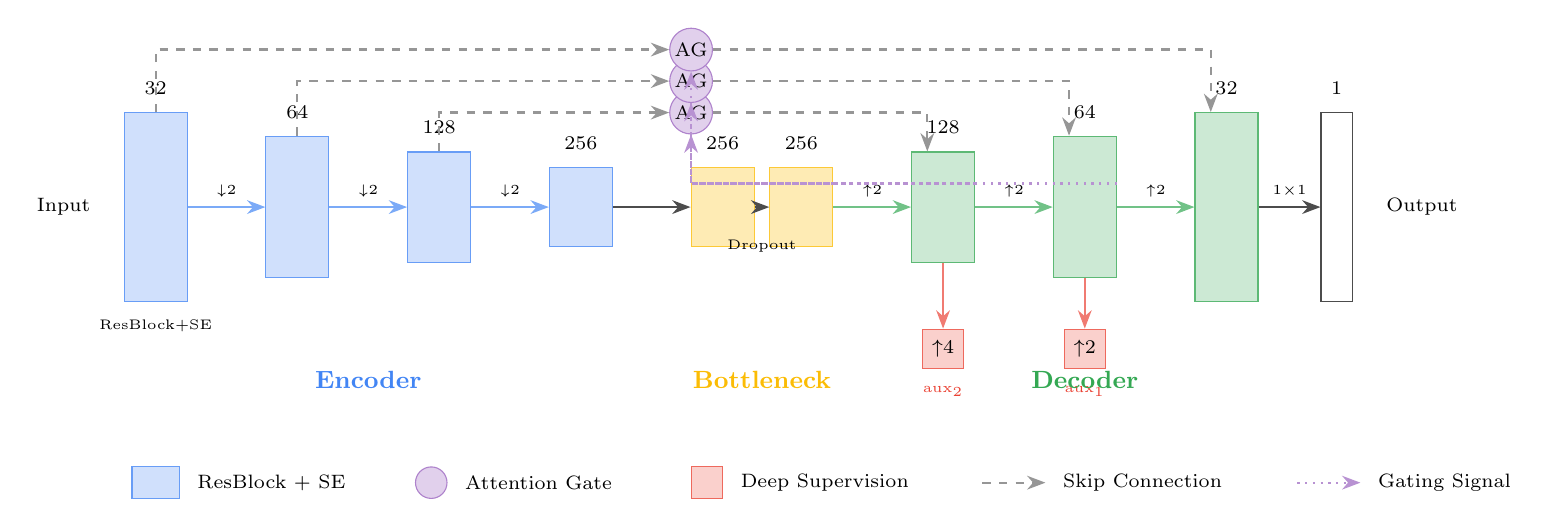
\begin{tikzpicture}[
    % Node styles
    encblock/.style={
        rectangle,
        draw=encoderblue!80,
        fill=encoderblue!25,
        minimum width=0.8cm,
        minimum height=#1,
        font=\footnotesize,
        inner sep=2pt,
    },
    decblock/.style={
        rectangle,
        draw=decodergreen!80,
        fill=decodergreen!25,
        minimum width=0.8cm,
        minimum height=#1,
        font=\footnotesize,
        inner sep=2pt,
    },
    bottleblock/.style={
        rectangle,
        draw=bottleneckorange!80,
        fill=bottleneckorange!30,
        minimum width=0.8cm,
        minimum height=#1,
        font=\footnotesize,
        inner sep=2pt,
    },
    attgate/.style={
        circle,
        draw=attentionpurple!80,
        fill=attentionpurple!30,
        minimum size=0.5cm,
        font=\scriptsize,
        inner sep=1pt,
    },
    dshead/.style={
        rectangle,
        draw=dsred!80,
        fill=dsred!25,
        minimum width=0.5cm,
        minimum height=0.5cm,
        font=\scriptsize,
    },
    % Arrow styles
    dataflow/.style={
        ->,
        >=Stealth,
        thick,
        draw=black!70,
    },
    skipconn/.style={
        ->,
        >=Stealth,
        thick,
        draw=skipgray,
        dashed,
    },
    downarrow/.style={
        ->,
        >=Stealth,
        thick,
        draw=encoderblue!70,
    },
    uparrow/.style={
        ->,
        >=Stealth,
        thick,
        draw=decodergreen!70,
    },
    % Label style
    blocklabel/.style={
        font=\scriptsize,
        text=black,
    },
]

% ============== ENCODER ==============
% Heights represent relative spatial size (decreasing)
\node[encblock=2.4cm] (enc0) at (0, 0) {};
\node[blocklabel, above=0.1cm of enc0] {32};
\node[blocklabel, below=0.1cm of enc0] {\tiny ResBlock+SE};

\node[encblock=1.8cm] (enc1) at (1.8, 0) {};
\node[blocklabel, above=0.1cm of enc1] {64};

\node[encblock=1.4cm] (enc2) at (3.6, 0) {};
\node[blocklabel, above=0.1cm of enc2] {128};

\node[encblock=1.0cm] (enc3) at (5.4, 0) {};
\node[blocklabel, above=0.1cm of enc3] {256};

% Downsampling arrows
\draw[downarrow] (enc0.east) -- node[above, font=\tiny] {$\downarrow$2} (enc1.west);
\draw[downarrow] (enc1.east) -- node[above, font=\tiny] {$\downarrow$2} (enc2.west);
\draw[downarrow] (enc2.east) -- node[above, font=\tiny] {$\downarrow$2} (enc3.west);

% ============== BOTTLENECK ==============
\node[bottleblock=1.0cm] (bottle1) at (7.2, 0) {};
\node[bottleblock=1.0cm] (bottle2) at (8.2, 0) {};
\node[blocklabel, above=0.1cm of bottle1] {256};
\node[blocklabel, above=0.1cm of bottle2] {256};
\node[blocklabel, below=0.3cm of $(bottle1)!0.5!(bottle2)$] {\tiny Dropout};

\draw[dataflow] (enc3.east) -- (bottle1.west);
\draw[dataflow] (bottle1.east) -- (bottle2.west);

% ============== DECODER ==============
\node[decblock=1.4cm] (dec2) at (10.0, 0) {};
\node[blocklabel, above=0.1cm of dec2] {128};

\node[decblock=1.8cm] (dec1) at (11.8, 0) {};
\node[blocklabel, above=0.1cm of dec1] {64};

\node[decblock=2.4cm] (dec0) at (13.6, 0) {};
\node[blocklabel, above=0.1cm of dec0] {32};

% Upsampling arrows
\draw[uparrow] (bottle2.east) -- node[above, font=\tiny] {$\uparrow$2} (dec2.west);
\draw[uparrow] (dec2.east) -- node[above, font=\tiny] {$\uparrow$2} (dec1.west);
\draw[uparrow] (dec1.east) -- node[above, font=\tiny] {$\uparrow$2} (dec0.west);

% ============== OUTPUT ==============
\node[rectangle, draw=black!70, fill=white, minimum width=0.4cm, minimum height=2.4cm] (output) at (15.0, 0) {};
\node[blocklabel, above=0.1cm of output] {1};
\draw[dataflow] (dec0.east) -- node[above, font=\tiny] {1$\times$1} (output.west);

% ============== ATTENTION GATES ==============
\node[attgate] (att2) at ($(enc2.east)!0.5!(dec2.west) + (0, 1.2)$) {AG};
\node[attgate] (att1) at ($(enc1.east)!0.5!(dec1.west) + (0, 1.6)$) {AG};
\node[attgate] (att0) at ($(enc0.east)!0.5!(dec0.west) + (0, 2.0)$) {AG};

% Skip connections (encoder to attention gate)
\draw[skipconn] (enc2.north) |- (att2.west);
\draw[skipconn] (enc1.north) |- (att1.west);
\draw[skipconn] (enc0.north) |- (att0.west);

% Attention gate to decoder
\draw[skipconn] (att2.east) -| ([xshift=-0.2cm]dec2.north);
\draw[skipconn] (att1.east) -| ([xshift=-0.2cm]dec1.north);
\draw[skipconn] (att0.east) -| ([xshift=-0.2cm]dec0.north);

% Gating signals (from decoder path to attention gates)
\draw[dataflow, dotted, draw=attentionpurple!70] ([yshift=0.3cm]bottle2.east) -| (att2.south);
\draw[dataflow, dotted, draw=attentionpurple!70] ([yshift=0.3cm]dec2.east) -| (att1.south);
\draw[dataflow, dotted, draw=attentionpurple!70] ([yshift=0.3cm]dec1.east) -| (att0.south);

% ============== DEEP SUPERVISION ==============
\node[dshead] (ds2) at (10.0, -1.8) {$\uparrow$4};
\node[dshead] (ds1) at (11.8, -1.8) {$\uparrow$2};

\draw[dataflow, draw=dsred!70] (dec2.south) -- (ds2.north);
\draw[dataflow, draw=dsred!70] (dec1.south) -- (ds1.north);

\node[blocklabel, below=0.1cm of ds2, text=dsred] {\tiny aux$_2$};
\node[blocklabel, below=0.1cm of ds1, text=dsred] {\tiny aux$_1$};

% ============== INPUT/OUTPUT LABELS ==============
\node[blocklabel, left=0.3cm of enc0] {Input};
\node[blocklabel, right=0.3cm of output] {Output};

% ============== SECTION LABELS ==============
\node[font=\small\bfseries, encoderblue] at (2.7, -2.2) {Encoder};
\node[font=\small\bfseries, bottleneckorange] at (7.7, -2.2) {Bottleneck};
\node[font=\small\bfseries, decodergreen] at (11.8, -2.2) {Decoder};

% ============== LEGEND ==============
\begin{scope}[shift={(0, -3.5)}]
    \node[encblock=0.4cm, minimum width=0.6cm] (leg1) at (0, 0) {};
    \node[blocklabel, right=0.1cm of leg1] {ResBlock + SE};

    \node[attgate, minimum size=0.4cm] (leg2) at (3.5, 0) {};
    \node[blocklabel, right=0.1cm of leg2] {Attention Gate};

    \node[dshead, minimum width=0.4cm, minimum height=0.4cm] (leg3) at (7, 0) {};
    \node[blocklabel, right=0.1cm of leg3] {Deep Supervision};

    \draw[skipconn] (10.5, 0) -- (11.3, 0);
    \node[blocklabel, right=0.1cm] at (11.3, 0) {Skip Connection};

    \draw[dataflow, dotted, draw=attentionpurple!70] (14.5, 0) -- (15.3, 0);
    \node[blocklabel, right=0.1cm] at (15.3, 0) {Gating Signal};
\end{scope}

\end{tikzpicture}
\end{document}
